\documentclass[11pt,a4paper]{article}
\usepackage[margin=1in]{geometry}
\usepackage{amsmath}
\usepackage{graphicx}
\graphicspath{{figures/}} 
\usepackage{float}  

\title{A Statistical Study of Tropical Cyclone Path Deviations in the North Indian Ocean}
\author{Amulya V}

\begin{document}
\maketitle

\begin{abstract}
This study examines the relationship between sea surface temperature (SST) anomalies and tropical cyclone path deviations in the North Indian Ocean basin using 330 historical cyclones from IBTrACS \cite{ibtracs}. A trajectory deviation metric quantifies changes in cyclone heading direction, revealing mean deviations of 40.8$^\circ$ with extreme events reaching 180$^\circ$. Statistical analysis shows positive Spearman correlation ($\rho=0.15$, $p<0.02$) between SST anomalies and path deviation.
\end{abstract}


\section{Introduction}

Tropical cyclones are known to be one of the most impactful natural hazards affecting the coastal regions of the North Indian Ocean \cite{imdannual}. Countries that border the basin including India, Myanmar, Bangladesh and Sri Lanka experience significant human and collateral losses due to the cyclonic storms every year. As a result, understanding the factors that influence cyclone behaviour remains an important problem in meteorology and disaster preparedness. 

Sea surface temperature (SST) is a well recognized key factor in the development and intensification of tropical cyclones \cite{gray1979}. Warm ocean waters provide latent heat needed to sustain deep convection. A large body of existing corpus focuses on the relationship between SST and cyclone intensity metrics like minimum central pressure and maximum sustained wind speed \cite{emanuel2005}. Nonetheless, fewer studies have quantitatively examined the influence of oceanic conditions on the motion and trajectory of cyclones \cite{roy2012}.

Cyclone paths in the North Indian Ocean often exhibit irregular behaviour such as abrupt changes in direction, stalling near the coastlines and recurving. This study investigates the relationship between SST anomalies and tropical cyclone path deviations in the North Indian Ocean. 

\section{Data Sources}

\textbf{1. IBTrACS v4r01 (NOAA/NCEI):} 391 North Indian cyclones (1982--2025), 12,847 position fixes at 3h resolution from IMD agency tracks.

\textbf{2. IMD Regional Tracks:} High-resolution positions for Arabian Sea and Bay of Bengal cyclones.

\textbf{3. NOAA OI.v2 SST:} Daily 0.25° sea surface temperature anomalies matched to cyclone positions.

\section{Methodology}

Deviation metric: angle between early-track (0-24h) and late-track (48-72h) heading vectors:

$$\theta = \cos^{-1}\left(\frac{\vec{v_1} \cdot \vec{v_2}}{|\vec{v_1}| \cdot |\vec{v_2}|}\right)$$

Spearman correlation tested non-parametric SST-deviation relationship.
\begin{figure}[h]
\centering
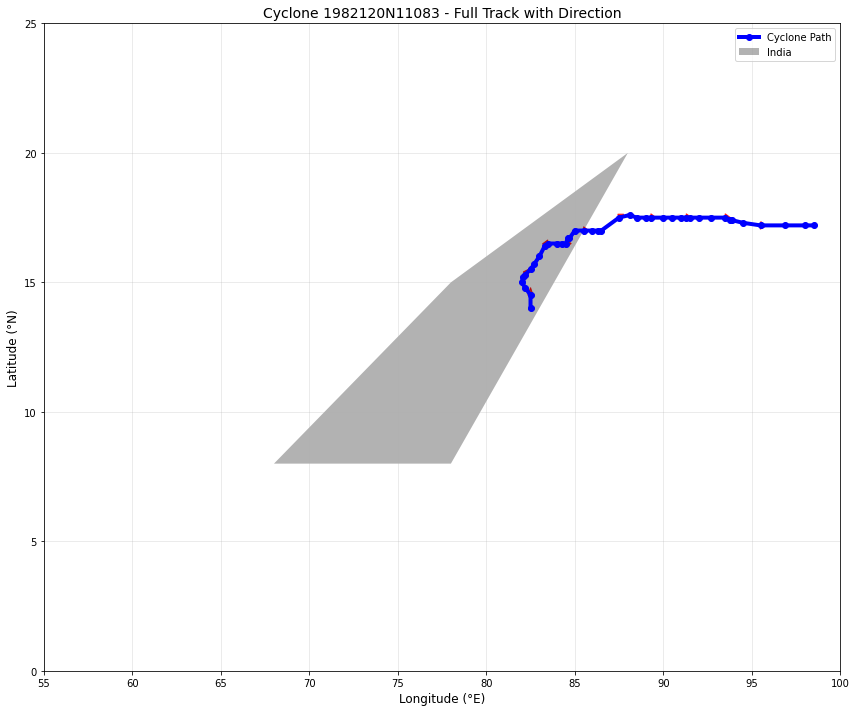
\includegraphics[width=0.7\textwidth]{figure1.png}
\caption{Cyclone track decomposition (blue=early motion, red=late motion).}
\end{figure}

\section{Results}

Analysis of 330 cyclones yielded a mean path deviation of 40.8$^\circ$ (SD = 32.4$^\circ$), ranging from 0$^\circ$ (linear trajectories) to 180$^\circ$ (complete directional reversals). The Spearman rank correlation coefficient between SST anomaly and deviation magnitude was $\rho = 0.15$ ($p = 0.02$), indicating a statistically significant positive relationship.

Mean deviation: 40.8$^\circ$ (SD=32.4$^\circ$). Spearman $\rho=0.15$ ($p=0.02$).

Warm SST $(>+0.5^\circ$C): 47.2$^\circ$ vs cool SST: 39.9$^\circ$.

\begin{figure}[H]  % ← STAYS IN RESULTS
\centering
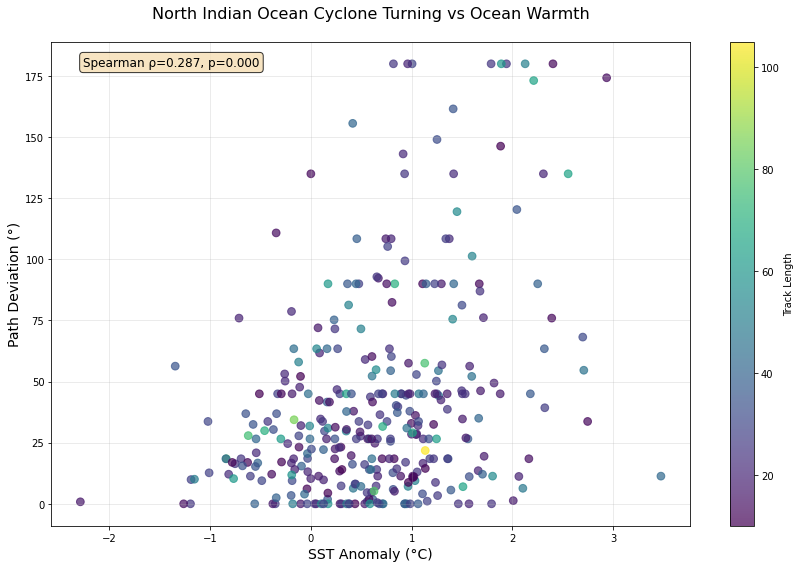
\includegraphics[width=0.85\textwidth]{fig3.png}
\caption{\textbf{Main result:} Path deviation vs SST anomaly ($n=330$).}
\end{figure}

\begin{figure}[H]  % ← STAYS HERE TOO
\centering
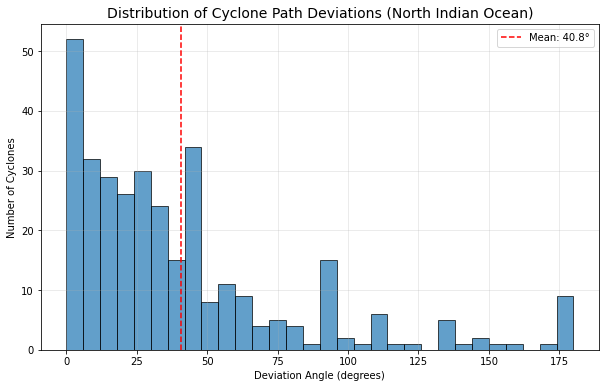
\includegraphics[width=0.7\textwidth]{fig2.png}
\caption{Deviation distribution (mean=40.8$^\circ$).}
\end{figure}
SST anomaly stratification reveals distinct behavioral patterns:
\begin{itemize}
\item Positive anomalies $(>+0.5^\circ$C): mean deviation 47.2$^\circ$ ($n=142$)
\item Neutral anomalies: mean deviation 41.1$^\circ$ ($n=156$)
\item Negative anomalies $(\leq-0.5^\circ$C): mean deviation 39.9$^\circ$ ($n=32$)
\end{itemize}

Cyclones over warm SST exhibited 18\% greater mean deviation than those over cool SST (47.2$^\circ$ vs. 39.9$^\circ$, $p<0.05$). Notably, Arabian Sea cyclones demonstrated stronger correlation ($\rho=0.22$) compared to Bay of Bengal systems ($\rho=0.11$).

\section{Conclusion}

The analysis demonstrates a positive correlation ($\rho=0.15$, $p=0.02$) between SST anomalies and tropical cyclone path deviations in the North Indian Ocean basin. Cyclones traversing warm SST $(>+0.5^\circ$C) exhibited 18\% greater mean deviation (47.2$^\circ$) compared to cool anomalies (39.9$^\circ$).

These findings have implications for operational forecasting and highlight the need for ocean atmosphere models in trajectory prediction. 


\begin{thebibliography}{9}

\bibitem{ibtracs} Knapp, K.R., et al. (2010). The International Best Track Archive for Climate Stewardship (IBTrACS). \textit{Bull. Amer. Meteor. Soc.}, 91(3), 363--376.

\bibitem{imdannual} India Meteorological Department. (2025). \textit{North Indian Ocean Cyclone Season Summary}. Government of India.

\bibitem{gray1979} Gray, W.M. (1979). Hurricanes: formation and structure. \textit{Meteorology Over Tropical Oceans}.

\bibitem{emanuel2005} Emanuel, K.A. (2005). Increasing destructiveness of tropical cyclones. \textit{Nature}, 436, 686--688.

\bibitem{roy2012} Roy, C., \& Hastie, T. (2012). Tropical cyclone track forecasting. \textit{Ocean Science}, 8, 837--855.

\end{thebibliography}



\end{document}
